% !TEX root = main.tex
\section{Design Description}
\label{sec:design_description}
Figure \ref{fig:block_toplevel} shows how the transmitter and receiver communicates within the system. Block diagrams for the two subsystems is shown in appendix \ref{a:block_diagram}, figure \ref{fig:block_diagram} and \ref{fig:block_diagram_feedback}. The data rate between each block is indicated with the thin arrows. The behaviour of the system will be explained in this section. 

Because two different modulation schemes are used, the receiver need to know how to decode the incoming data packets. This problem is solved by using two different training sequences, both of length \barkerSymbols\   symbols. The training sequence is an appropriate repetition of barker sequences of length 7 and 13, for QPSK and QAM-64 modulation respectively. As shown in figure \ref{fig:block_diagram}, after frame sync, the receiver perform a check on the received barker sequence before de-mapping the symbols. 

In the transmitter, a variable called \textit{Session State} keep the information about what data quality and modulation scheme to use. As figure \ref{fig:block_diagram} indicates, the session state influences several blocks of the TX side of the transmitter. The decision of when to change data quality is left completely to the transmitter. For every received data package, the receiver computes the number of detected errors and transmit this number back to the transmitter. These BER packages are always transmitted using QPSK-modulation. Based on the received number of detected errors as well as previous error detections, the transmitter decides whether to change session state or not. 

The sound producer and sound consumer contains functionality for handling the sound input and output to the sound card of the computer. They are implemented using the Windows API \cite{WinAPI}. Sound producer reads sound samples from the sound card at full quality (16 bit, 44100 Hz stereo) and writes the samples to a queue accessible for the source encoder. Sound consumer equivalently reads sound samples from a queue controlled by the unpacking block and writes to the computer sound card. 

The source encoder performs lossy compression of the produced sound samples. The bit resolution is reduced to 12 bit per sound sample, and the sampling rate is reduced by a factor 2 or 4 depending on the session state. The source decoder performs the inverse operation, writing 2 or 4 copies of the same sample to the sound consumer.  

In the packing block, sound data is read from the source encoder, a header is added, and the packet is sent to the packet queue. The eight bit packet header consist of a three bit session ID and a five bit packet ID. 

A scrambler is implemented before FEC, which computes a bitwise XOR between a pseudo random bit string and the packet. The bit string used for scrambling is of the same size as the packet itself. The scrambler performs the exact same operation at RX and TX.

The implemented FEC algorithm is Hamming (7,4). The implementation is a fast, pre-written C-code, written by Michael Dipperstein \cite{hamming}. 

The system uses Grey Code for mapping the binary data to a complex vector $z$. The mapping schemes are shown in figure \ref{fig:mapping}.

% !TEX root = main.tex
\begin{figure} 
    \centering
  \subfloat[\label{1a}]{%
  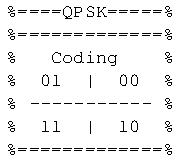
\includegraphics[width=0.3\linewidth]{qpsk_mapping.pdf}
  
}
\\ 
  \subfloat[\label{1b}]{%
    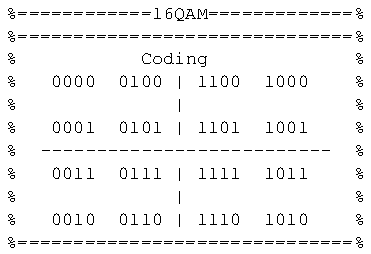
\includegraphics[width=0.6\linewidth]{qam16mapping.pdf}
}

  \caption{Symbol mapping for QPSK (a) and QAM-16 (b) modulated symbols}
  \label{fig:mapping} 
\end{figure}


The training sequence is added to both I and Q symbols in the block \textit{Add Barker}. As previously described, the training sequence is a barker sequence of length 7 or 13 depending on the session state. In either case the total length of the training sequence is \barkerSymbols symbols, which means that the barker sequence is repeated to obtain the desired length. 

In the last step before transmission, the symbols are upsampled by a factor $\sps$ and filtered with a pulse shaping filter. The filter is Root Raised Cosine with a roll-off factor of 0.3. The same filter is applied as a matched filter in the first step at the receive side before the samples are downsampled again. 

The USRP is configured to transmit continuously with a symbol rate of $\symbolRateQPSK$ symbols per second and transmit arrays of zeros when no data is available. The USRP interface is implemented using the NI-USRP DLL \cite{labviewDLL}.

Symbol synchronisation is done by choosing the sample offset that maximizes the signal energy. 

Frame synchronisation is done by computing the crosscorrelation between the two training sequences and the received symbols. The value of the crosscorrelation is compared to a pre set threshold. The first index that gives a value exceeding this threshold is considered to be the beginning of the frame. After a frame is found, only the frame symbols are passed along to the next block.

\subsection{Frequency and Phase Synchronisation}
The implemented frequency synchronisation algorithm is based on the Mth-power algorithm, which is further improved by using a Kalman filter. Frequency offset is estimated from the training sequence only. The Mth-power algorithm estimates the phase offset of MPSK modulated symbols, by mapping all symbols to the same point in the complex plane. By tracking the angular difference between consecutive symbols, the frequency offset may be estimated. In our case, the QPSK symbols of the training sequence is raised to the 4th power, and the phase is estimated as indicated in figure \ref{fig:mth_pow}.
% !TEX root = main.tex
\begin{figure}[htbp]
\centering
\begin{tikzpicture}
% Grids
\coordinate (origo) at (0,0);
\coordinate (origo_w) at (5.1,0);

\draw[step=0.3cm,gray,very thin] (-1.51,-1.51) grid (1.5,1.5);
\draw[step=0.3cm,gray,very thin] (3.6,-1.51) grid (6.6, 1.5);

% Axis
\draw[thick, ->] (-1.5,0) -- (1.5, 0) node [anchor=north west]{\Re[$z$]};
\draw[thick, ->] (0,-1.5) -- (0,1.5) node [anchor=south west]{\Im[$z$]};
\draw[thick, ->] (3.6,0) -- (6.6, 0) node [anchor=north west]{\Re[$w$]};
\draw[thick, ->] (5.1,-1.5) -- (5.1,1.5) node [anchor=south west]{\Im[$w$]};

\draw[thick] (0.9, 0) ++(0, 2pt) -- ++(0,-4pt) node[font=\scriptsize, yshift=-0.1cm, xshift=-0.1cm]{1};
\draw[thick] (-0.9, 0) ++(0, 2pt) -- ++(0,-4pt) node[font=\scriptsize, yshift=-0.1cm, xshift=-0.1cm]{-1};
\draw[thick] (0, 0.9) ++(2pt, 0) -- ++(-4pt, 0) node[font=\scriptsize, yshift=-0.1cm, xshift=-0.1cm]{1};
\draw[thick] (0, -0.9) ++(2pt, 0) -- ++(-4pt, 0) node[font=\scriptsize, yshift=-0.1cm, xshift=-0.1cm]{-1};

\draw[thick] (6, 0) ++(0, 2pt) -- ++(0,-4pt) node[font=\scriptsize, yshift=-0.1cm, xshift=-0.1cm]{4};
\draw[thick] (4.2, 0) ++(0, 2pt) -- ++(0,-4pt) node[font=\scriptsize, yshift=-0.1cm, xshift=-0.1cm]{-4};
\draw[thick] (5.1, 0.9) ++(2pt, 0) -- ++(-4pt, 0) node[font=\scriptsize, yshift=-0.1cm, xshift=-0.1cm]{4};
\draw[thick] (5.1, -0.9) ++(2pt, 0) -- ++(-4pt, 0) node[font=\scriptsize, yshift=-0.1cm, xshift=-0.1cm]{-4};

% Plot
\draw[blue,fill=blue] (0.9,0.9) circle (2pt) coordinate[](sample);
\draw[blue,fill=blue] (-0.9,0.9) circle (2pt);
\draw[blue,fill=blue] (0.9,-0.9) circle (2pt);
\draw[blue,fill=blue] (-0.9,-0.9) circle (2pt);
\draw[red,fill=red] (0.73,1.043) circle (2pt) coordinate[](sample_err);

\draw[thin, blue] (0,0) -- (sample);
\draw[thin, red] (0,0) -- (sample_err);
\pic [draw, red, ->, angle eccentricity=1.5] {angle = sample--origo--sample_err};
\draw (0.3, 0.3) node[anchor=north west, text=red, yshift=0.2cm]{$\phi$};

\draw[blue,fill=blue] (3.83,0) circle (2pt) coordinate[](sample_w);
\draw[red,fill=red] (4.125,-0.818) circle (2pt) coordinate[](sample_err_w);
\draw[thin, blue] (origo_w) -- (sample_w);
\draw[thin, red] (origo_w) -- (sample_err_w);
\pic [draw, red, ->, angle eccentricity=1.5] {angle = sample_w--origo_w--sample_err_w};
\draw (origo_w) ++(-1.1,-0.35) node[anchor=north west, text=red, yshift=0.2cm]{$4\phi$};

% Other
\draw[thick, ->] (2, 1) .. controls (2.5,1.1) .. (3,1) node[above, anchor=south east, xshift=0.1cm]{$w=z^4$} ;

\end{tikzpicture}
\caption{Illustration the mapping $w=z^4$ which indicates how a phase error in QPSK modulated signal can be observed.}
\label{fig:mth_pow}
\end{figure}

For each received frame, the frequency offset is estimated by the mean of the angular difference between all consecutive symbols of the training sequence. The estimate obtained from a single frame at time $k$  is referred to as $\widetilde{\omega}_k$.  

The accuracy of the estimate is improved by using a Kalman filter. The state of the Kalman filter is the one-dimensional state vector $\omega_k$ which is the true frequency offset between the transmitter and the receiver at time $k$ (i.e. frame $k$). The state is represented by the \textit{a posteriori} state and variance estimate $\widehat{\omega}_{k | k}$ and $\widehat{\sigma}_{k | k}$, where the subscript $n | m$ indicates the estimate of time $n$ given observations up to and including time $m \leq n$. 

The estimate is obtained in two stages, referred to as the \textit{prediction stage} and the \textit{update stage}. In the prediction stage, the \textit{a priori} estimates $\widehat{\omega}_{k | k-1}$ and $\widehat{\sigma}_{k | k-1}$ is obtained by equations \ref{eq:kalman_pred_wk} and \ref{eq:kalman_pred_sigmak}. $\sigma_f$ is the stationary variance of the process noise and must be tuned carefully in order to obtain appropriate convergence speed. In our system $\sigma_f$ was set to $0.8\cdot 10^{-6}$.  

\begin{gather}
\widehat{\omega}_{k | k-1} = \widehat{\omega}_{k-1 | k-1}  \label{eq:kalman_pred_wk} \\
\widehat{\sigma}_{k | k-1} = \widehat{\sigma}_{k-1 | k-1} + \sigma_f \label{eq:kalman_pred_sigmak} 
\end{gather} 

In the update stage, the \textit{a posteriori} estimates $\widehat{\omega}_{k | k}$ and $\widehat{\sigma}_{k | k}$ is obtained by equations \ref{eq:kalman_up_wk} and \ref{eq:kalman_up_sigmak}. $\widetilde{\omega}_k$ and $\widetilde{\sigma}_{k}$ is the observed frequency offset and estimated observation noise at time $k$ respectively.

\begin{gather}
\widehat{\omega}_{k | k} = \widehat{\omega}_{k | k-1} + \frac{\widehat{\sigma}_{k | k-1}}{\widehat{\sigma}_{k | k-1} + \widetilde{\sigma}_{k}} ( \widetilde{\omega}_{k} - \widehat{\omega}_{k | k-1} )  \label{eq:kalman_up_wk} \\
\widehat{\sigma}_{k | k} = \widehat{\sigma}_{k | k-1} \frac{\widetilde{\sigma}_{k}}{\widetilde{\sigma}_{k} + \widehat{\sigma}_{k | k-1}  } \label{eq:kalman_up_sigmak} 
\end{gather} 

After the estimates $\widehat{\omega}_{k | k}$ and $\widehat{\sigma}_{k | k}$ is obtained, $\widehat{\omega}_{k | k}$ is applied to each symbol in frame $k$. The phase offset is then estimated as the mean of the angular deviation between the training sequence of the received symbols, and the ideal barker sequence.


